%中間審査概要テンプレート ver. 3.0

\documentclass[uplatex,twocolumn,dvipdfmx]{jsarticle}
\usepackage[top=22mm,bottom=22mm,left=22mm,right=22mm]{geometry}
\setlength{\columnsep}{10mm}
\usepackage[T1]{fontenc}
\usepackage{txfonts}
\usepackage[expert,deluxe]{otf}
\usepackage[dvipdfmx,hiresbb]{graphicx}
\usepackage[dvipdfmx]{hyperref}
\usepackage{pxjahyper}
\usepackage{secdot}





%タイトルと学生番号,名前だけ編集すること
\title{\vspace{-5mm}\fontsize{14pt}{0pt}\selectfont 文書自動添削システムによる学生の文書改善履歴の調査}
\author{\normalsize プロジェクトマネジメントコース 矢吹研究室 1442031 氏名 小山隆太郎}
\date{}
\pagestyle{empty}
\begin{document}
\fontsize{10.5pt}{\baselineskip}\selectfont
\maketitle





%以下が本文
\section{背景}
学生が行う研究では,研究だけではなく文書を作成する時間が多い.特に卒業論文は文量も多く,形式も指定されるため,文書校正にかかる労力は大きい.また,自分以外が読んでもわかりやすい文書を書く必要があり,文が長いほど理解が難しくなってしまう場合や,「だから」,「かなり」といった口語が混じり,文書の質が落ちてしまうことがある.

このような状況にRedPen\cite{a}を執筆環境に導入することで,文書の質が向上することが期待されている.RedPenは技術文書をターゲットにした文書自動添削ツールであり,現在もコードの追加,改変が行われている.

\section{目的}
RedPenは学校や会社等の組織のルールに対応できるように設定が柔軟に行える仕様になっている.マシンを用いた文書添削を繰り返し行い,論文向けの添削システムを確立し,文書の質の向上と,作成時間の短縮を図ることを目的とする.

\section{手法}
添削システムに必要な要素を以下の手法で調査する.

\begin{enumerate}
 \item 執筆中の文書の添削に,CI(継続的インテグレーション)サーバを導入する.GitHubに提出した文書の添削を自動で行い,エラー内容を瞬時に確認できるようにする.文書を提出する度にエラー内容を集める\cite{b}.
 \item 集めた添削結果から添削システムに必要な要素を考察し,RedPenのコードを追加,改変する.
\end{enumerate}

\section{想定される成果物}
個人,複数人プロジェクトで活用できる文書添削システムを構築する.

\section{進捗状況}
矢吹研究室に所属する3年生の課題文を,文長に関する添削機能(SentenceLength,CommaNumber,InvalidSymbol)や,文書表現に関する機能(InvalidWord,InvalidExpression)を用いて添削した.一文が長い文や,数値や専門用語の表現が統一されていないことを抑える設定で行い,図\ref{conf}の推移結果を得た.

\begin{figure}[h]
\centering
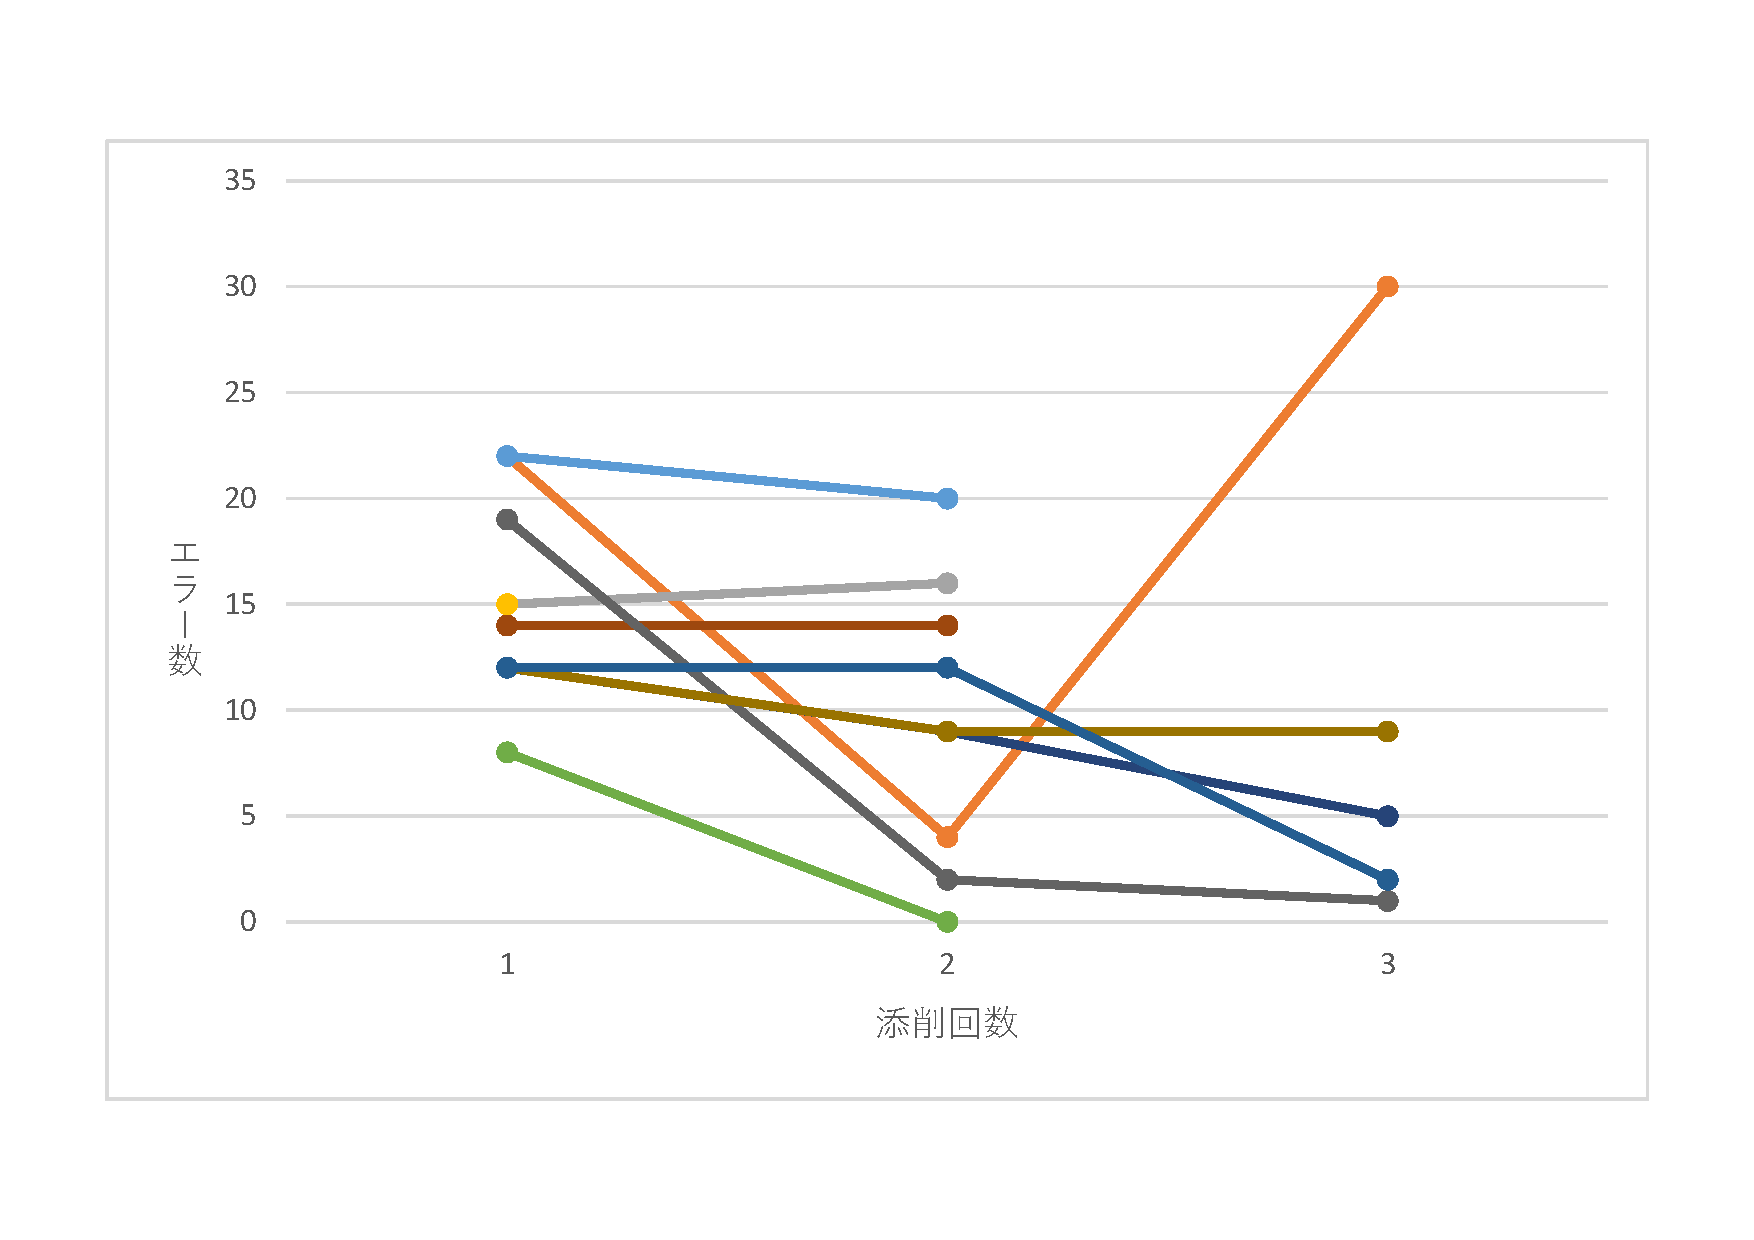
\includegraphics[width=8cm,clip]{images.pdf}
\caption{添削項数の推移}\label{conf}
\end{figure}

添削結果から,エラー数が減っている文書は,執筆の度に文が短くなる特徴が得られた.

エラー数が減らない文書には,カンマや助詞が多いままの文書が見受けられた.また,添削システムの設定が不十分であることも要因である.



\section{今後の計画}
論文に適切な文長や表現等の要素を考察し,添削機能の追加,改変を行い機能を実装する.文書作成に利用してもらう.


\bibliographystyle{junsrt}
\bibliography{biblio}%「biblio.bib」というファイルが必要.

\end{document}
